\documentclass{beamer}
\beamertemplatenavigationsymbolsempty
\usecolortheme{beaver}
\setbeamertemplate{blocks}[rounded=true, shadow=true]
\setbeamertemplate{footline}[page number]

\usepackage{amsmath,amssymb,amsfonts}
\usepackage{graphicx}
\usepackage{tikz}
\usepackage{booktabs}

\title{Subspace Inference for Bayesian Deep Learning}
\author{Pavel Izmailov, Wesley J. Maddox, Polina Kirichenko, \\ Timur Garipov, Dmitry Vetrov, Andrew Gordon Wilson}
\institute{Talk by Dmitrii Vasilenko}
\date{\today}

\begin{document}

\begin{frame}
\titlepage
\end{frame}

%----------------------
\begin{frame}{Problem: Bayesian Inference in Deep Learning}
\begin{itemize}
    \item Bayesian methods provide accurate predictive distributions and well-calibrated uncertainty
    \item But modern DNNs have extremely high-dimensional parameter spaces ($\sim 10^6 - 10^9$)
    \item Standard Bayesian inference (MCMC, VI) doesn't scale well
    \item \textbf{Challenge:} How to perform efficient Bayesian inference in high-dimensional spaces?
\end{itemize}
\end{frame}

%----------------------
\begin{frame}{Key Idea: Subspace Inference (SI)}
Instead of working in the full parameter space $\mathbb{R}^d$:
\begin{block}{Subspace parameterization}
\[
w = \hat{w} + Pz, \quad z \in \mathbb{R}^K, \quad K \ll d
\]
where:
\begin{itemize}
    \item $\hat{w}$: shift vector
    \item $P$: projection matrix defining the subspace
    \item $z$: low-dimensional parameters for inference
\end{itemize}
\end{block}

\begin{figure}
    \begin{columns}
        \column{0.3\textwidth}
        \centering
        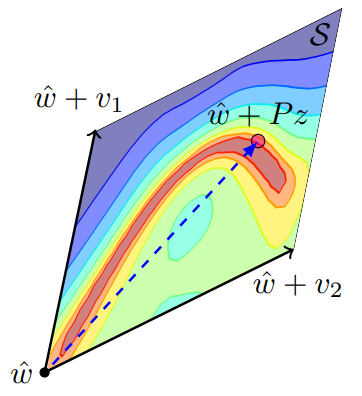
\includegraphics[width=\textwidth]{subspace_visualization.png}
        
        \column{0.4\textwidth}
        \caption{Illustration of subspace $\mathcal{S}$ with shift vector $\hat{w}$ and basis vectors $v_1$, $v_2$}
    \end{columns}
\end{figure}
\end{frame}

\begin{frame}{Bayesian Model Averaging in the Subspace}
\[
p(D \mid z) = p_M(D \mid w = \hat{w} + P z)
\]

\[
p(D^* \mid D) \approx \frac{1}{J} \sum_{j=1}^{J} p_M(D^* \mid \hat{w} + P z_j), \quad z_j \sim p(z \mid D)
\]
\begin{itemize}
    \item Draw $J$ samples from the posterior $p(z|D)$.
    \item Each sample $z_j$ defines a new model $w_j = \hat{w} + P z_j$.
    \item Average predictions → uncertainty-aware predictions.
\end{itemize}
\end{frame}

%----------------------
\begin{frame}{How to Construct the Subspace?}
Three main approaches:
\begin{enumerate}
    \item \textbf{Random subspace:} Simple but uninformative
    \item \textbf{PCA subspace:} From SGD trajectory
    \item \textbf{Curve subspace:} Connects multiple solutions along low-loss curve
\end{enumerate}
\end{frame}

\begin{frame}{Random Subspace}

\begin{itemize}
\item Sample $K$ random vectors: $v_i \sim \mathcal{N}(0,I)$
\item Normalize to unit length
\item Use stochastic weight averaging solution as base: $\hat{w} = w_{SWA}$
\end{itemize}

\begin{block}{Pros \& Cons}
\begin{itemize}
\item \textbf{+} Virtually free to construct
\item \textbf{+} Simple baseline
\item \textbf{-} Poor model diversity
\item \textbf{-} Uncertainty doesn't grow away from data
\end{itemize}
\end{block}

\end{frame}

\begin{frame}{PCA Subspace from SGD}

\begin{block}{Construction Steps}
1. Start from pretrained model \\
2. Run SGD with high LR \\
3. Collect weight snapshots $w_i$ \\
4. Compute SWA: $\hat{w} = \text{mean}(w_i)$ \\
5. PCA on deviations: $a_i = \hat{w} - w_i$ \\
6. Take first $K$ components as $P$
\end{block}

\begin{block}{Why it works}
SGD's oscillations reveal important directions. First PCA components align with top Hessian eigenvectors.
\end{block}

\end{frame}

\begin{frame}{Curve Subspace}
\begin{columns}
\column{0.4\textwidth}
\centering
\includegraphics[width=\textwidth]{curve_subspace.png}

\column{0.6\textwidth}
\begin{block}{Key Idea}
Connect two independent models with a low-loss curve in weight space.
\end{block}

\begin{block}{Basis Construction}
\begin{itemize}
\item Train two models: $w_0$ and $w_1$
\item Find curve $w(t)$ with low loss between them
\item $\hat{w} = (w_0 + w_1)/2$
\item $v_1 = (w_0 - \hat{w})/\|w_0 - \hat{w}\|$
\item $v_2 = (w_{1/2} - \hat{w})/\|w_{1/2} - \hat{w}\|$
\end{itemize}
\end{block}
\end{columns}

\begin{block}{Pros \& Cons}
\begin{itemize}
\item \textbf{+} Excellent accuracy
\item \textbf{-} Expensive (3× training cost)
\item \textbf{-} Fixed 2D subspace
\end{itemize}
\end{block}
\end{frame}

\begin{frame}{Bayesian Inference in the Subspace}


\begin{block}{Tempered posterior}
To prevent over-concentration:
\[
p_T(z|\mathcal{D}) \propto p(\mathcal{D}|z)^{1/T} p(z)
\]
\begin{itemize}
    \item $T=1$: original posterior
    \item $T \to \infty$: approaches prior
    \item Chosen via cross-validation
\end{itemize}
\end{block}
\end{frame}

%----------------------
\begin{frame}{Experiments: Regression (UCI Datasets)}
\begin{figure}
    \centering
    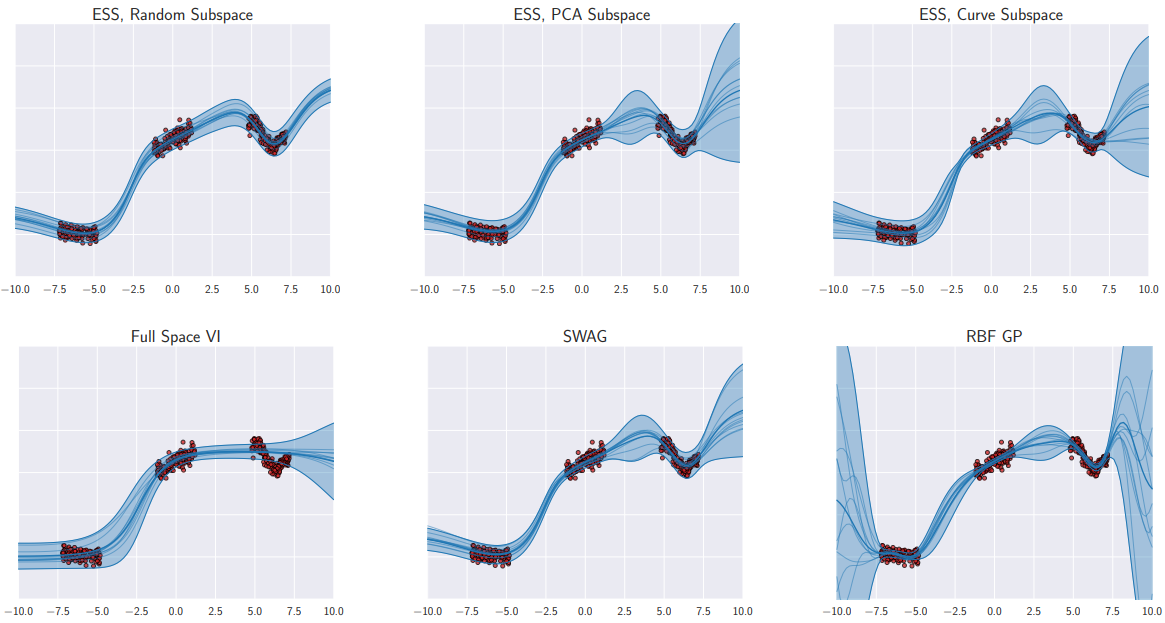
\includegraphics[width=0.85\textwidth]{regression_results.png}
    \caption{Predictive distributions for synthetic regression}
\end{figure}
\textbf{Key observation:} PCA and curve subspaces show uncertainty growing away from data.
\end{frame}

%----------------------
\begin{frame}{Experiments: Image Classification (CIFAR)}
\begin{table}[h]
\centering
\begin{tabular}{lcc}
\toprule
\textbf{Subspace} & \textbf{NLL} $\downarrow$ & \textbf{Accuracy} $\uparrow$ \\
\midrule
Random (10D) & $0.6858 \pm 0.0052$ & $80.17 \pm 0.03\%$ \\
PCA (10D) & $\mathbf{0.6652 \pm 0.004}$ & $\mathbf{80.54 \pm 0.13\%}$ \\
Curve (2D) & $\mathbf{0.6493 \pm 0.01}$ & $\mathbf{81.55 \pm 0.26\%}$ \\
\bottomrule
\end{tabular}
\caption{Results for PreResNet-164 on CIFAR-100}
\end{table}
\vspace{0.3cm}
\begin{itemize}
    \item Even 2D curve subspace improves performance
    \item PCA subspace offers good trade-off between cost and performance
\end{itemize}
\end{frame}

%----------------------
\begin{frame}{Conclusion}
\begin{itemize}
    \item Subspace Inference enables practical Bayesian deep learning
    \item Key insight: low-dimensional subspaces contain diverse, high-performing models
    \item PCA of SGD trajectory provides efficient, informative subspaces
    \item Method improves accuracy, calibration, and interpretability
    \item Bridge between SGD training and full Bayesian inference
\end{itemize}

\end{frame}


\end{document}